% !TeX spellcheck = en_US

%% bare_jrnl_compsoc.tex
%% V1.4b
%% 2015/08/26
%% by Michael Shell
%% See:
%% http://www.michaelshell.org/
%% for current contact information.
%%
%% This is a skeleton file demonstrating the use of IEEEtran.cls
%% (requires IEEEtran.cls version 1.8b or later) with an IEEE
%% Computer Society journal paper.
%%
%% Support sites:
%% http://www.michaelshell.org/tex/ieeetran/
%% http://www.ctan.org/pkg/ieeetran
%% and
%% http://www.ieee.org/

%%*************************************************************************
%% Legal Notice:
%% This code is offered as-is without any warranty either expressed or
%% implied; without even the implied warranty of MERCHANTABILITY or
%% FITNESS FOR A PARTICULAR PURPOSE! 
%% User assumes all risk.
%% In no event shall the IEEE or any contributor to this code be liable for
%% any damages or losses, including, but not limited to, incidental,
%% consequential, or any other damages, resulting from the use or misuse
%% of any information contained here.
%%
%% All comments are the opinions of their respective authors and are not
%% necessarily endorsed by the IEEE.
%%
%% This work is distributed under the LaTeX Project Public License (LPPL)
%% ( http://www.latex-project.org/ ) version 1.3, and may be freely used,
%% distributed and modified. A copy of the LPPL, version 1.3, is included
%% in the base LaTeX documentation of all distributions of LaTeX released
%% 2003/12/01 or later.
%% Retain all contribution notices and credits.
%% ** Modified files should be clearly indicated as such, including  **
%% ** renaming them and changing author support contact information. **
%%*************************************************************************


% *** Authors should verify (and, if needed, correct) their LaTeX system  ***
% *** with the testflow diagnostic prior to trusting their LaTeX platform ***
% *** with production work. The IEEE's font choices and paper sizes can   ***
% *** trigger bugs that do not appear when using other class files.       ***                          ***
% The testflow support page is at:
% http://www.michaelshell.org/tex/testflow/


\documentclass[10pt,journal,compsoc]{IEEEtran}
%
% If IEEEtran.cls has not been installed into the LaTeX system files,
% manually specify the path to it like:
% \documentclass[10pt,journal,compsoc]{../sty/IEEEtran}





% Some very useful LaTeX packages include:
% (uncomment the ones you want to load)


% *** MISC UTILITY PACKAGES ***
%
%\usepackage{ifpdf}
% Heiko Oberdiek's ifpdf.sty is very useful if you need conditional
% compilation based on whether the output is pdf or dvi.
% usage:
% \ifpdf
%   % pdf code
% \else
%   % dvi code
% \fi
% The latest version of ifpdf.sty can be obtained from:
% http://www.ctan.org/pkg/ifpdf
% Also, note that IEEEtran.cls V1.7 and later provides a builtin
% \ifCLASSINFOpdf conditional that works the same way.
% When switching from latex to pdflatex and vice-versa, the compiler may
% have to be run twice to clear warning/error messages.






% *** CITATION PACKAGES ***
%
\ifCLASSOPTIONcompsoc
  % IEEE Computer Society needs nocompress option
  % requires cite.sty v4.0 or later (November 2003)
  \usepackage[nocompress]{cite}
\else
  % normal IEEE
  \usepackage{cite}
\fi
% cite.sty was written by Donald Arseneau
% V1.6 and later of IEEEtran pre-defines the format of the cite.sty package
% \cite{} output to follow that of the IEEE. Loading the cite package will
% result in citation numbers being automatically sorted and properly
% "compressed/ranged". e.g., [1], [9], [2], [7], [5], [6] without using
% cite.sty will become [1], [2], [5]--[7], [9] using cite.sty. cite.sty's
% \cite will automatically add leading space, if needed. Use cite.sty's
% noadjust option (cite.sty V3.8 and later) if you want to turn this off
% such as if a citation ever needs to be enclosed in parenthesis.
% cite.sty is already installed on most LaTeX systems. Be sure and use
% version 5.0 (2009-03-20) and later if using hyperref.sty.
% The latest version can be obtained at:
% http://www.ctan.org/pkg/cite
% The documentation is contained in the cite.sty file itself.
%
% Note that some packages require special options to format as the Computer
% Society requires. In particular, Computer Society  papers do not use
% compressed citation ranges as is done in typical IEEE papers
% (e.g., [1]-[4]). Instead, they list every citation separately in order
% (e.g., [1], [2], [3], [4]). To get the latter we need to load the cite
% package with the nocompress option which is supported by cite.sty v4.0
% and later. Note also the use of a CLASSOPTION conditional provided by
% IEEEtran.cls V1.7 and later.





% *** GRAPHICS RELATED PACKAGES ***
%
\ifCLASSINFOpdf
  % \usepackage[pdftex]{graphicx}
  % declare the path(s) where your graphic files are
  % \graphicspath{{../pdf/}{../jpeg/}}
  % and their extensions so you won't have to specify these with
  % every instance of \includegraphics
  % \DeclareGraphicsExtensions{.pdf,.jpeg,.png}
\else
  % or other class option (dvipsone, dvipdf, if not using dvips). graphicx
  % will default to the driver specified in the system graphics.cfg if no
  % driver is specified.
  % \usepackage[dvips]{graphicx}
  % declare the path(s) where your graphic files are
  % \graphicspath{{../eps/}}
  % and their extensions so you won't have to specify these with
  % every instance of \includegraphics
  % \DeclareGraphicsExtensions{.eps}
\fi
% graphicx was written by David Carlisle and Sebastian Rahtz. It is
% required if you want graphics, photos, etc. graphicx.sty is already
% installed on most LaTeX systems. The latest version and documentation
% can be obtained at: 
% http://www.ctan.org/pkg/graphicx
% Another good source of documentation is "Using Imported Graphics in
% LaTeX2e" by Keith Reckdahl which can be found at:
% http://www.ctan.org/pkg/epslatex
%
% latex, and pdflatex in dvi mode, support graphics in encapsulated
% postscript (.eps) format. pdflatex in pdf mode supports graphics
% in .pdf, .jpeg, .png and .mps (metapost) formats. Users should ensure
% that all non-photo figures use a vector format (.eps, .pdf, .mps) and
% not a bitmapped formats (.jpeg, .png). The IEEE frowns on bitmapped formats
% which can result in "jaggedy"/blurry rendering of lines and letters as
% well as large increases in file sizes.
%
% You can find documentation about the pdfTeX application at:
% http://www.tug.org/applications/pdftex






% *** MATH PACKAGES ***
%
%\usepackage{amsmath}
% A popular package from the American Mathematical Society that provides
% many useful and powerful commands for dealing with mathematics.
%
% Note that the amsmath package sets \interdisplaylinepenalty to 10000
% thus preventing page breaks from occurring within multiline equations. Use:
%\interdisplaylinepenalty=2500
% after loading amsmath to restore such page breaks as IEEEtran.cls normally
% does. amsmath.sty is already installed on most LaTeX systems. The latest
% version and documentation can be obtained at:
% http://www.ctan.org/pkg/amsmath





% *** SPECIALIZED LIST PACKAGES ***
%
%\usepackage{algorithmic}
% algorithmic.sty was written by Peter Williams and Rogerio Brito.
% This package provides an algorithmic environment fo describing algorithms.
% You can use the algorithmic environment in-text or within a figure
% environment to provide for a floating algorithm. Do NOT use the algorithm
% floating environment provided by algorithm.sty (by the same authors) or
% algorithm2e.sty (by Christophe Fiorio) as the IEEE does not use dedicated
% algorithm float types and packages that provide these will not provide
% correct IEEE style captions. The latest version and documentation of
% algorithmic.sty can be obtained at:
% http://www.ctan.org/pkg/algorithms
% Also of interest may be the (relatively newer and more customizable)
% algorithmicx.sty package by Szasz Janos:
% http://www.ctan.org/pkg/algorithmicx




% *** ALIGNMENT PACKAGES ***
%
%\usepackage{array}
% Frank Mittelbach's and David Carlisle's array.sty patches and improves
% the standard LaTeX2e array and tabular environments to provide better
% appearance and additional user controls. As the default LaTeX2e table
% generation code is lacking to the point of almost being broken with
% respect to the quality of the end results, all users are strongly
% advised to use an enhanced (at the very least that provided by array.sty)
% set of table tools. array.sty is already installed on most systems. The
% latest version and documentation can be obtained at:
% http://www.ctan.org/pkg/array


% IEEEtran contains the IEEEeqnarray family of commands that can be used to
% generate multiline equations as well as matrices, tables, etc., of high
% quality.




% *** SUBFIGURE PACKAGES ***
%\ifCLASSOPTIONcompsoc
%  \usepackage[caption=false,font=footnotesize,labelfont=sf,textfont=sf]{subfig}
%\else
%  \usepackage[caption=false,font=footnotesize]{subfig}
%\fi
% subfig.sty, written by Steven Douglas Cochran, is the modern replacement
% for subfigure.sty, the latter of which is no longer maintained and is
% incompatible with some LaTeX packages including fixltx2e. However,
% subfig.sty requires and automatically loads Axel Sommerfeldt's caption.sty
% which will override IEEEtran.cls' handling of captions and this will result
% in non-IEEE style figure/table captions. To prevent this problem, be sure
% and invoke subfig.sty's "caption=false" package option (available since
% subfig.sty version 1.3, 2005/06/28) as this is will preserve IEEEtran.cls
% handling of captions.
% Note that the Computer Society format requires a sans serif font rather
% than the serif font used in traditional IEEE formatting and thus the need
% to invoke different subfig.sty package options depending on whether
% compsoc mode has been enabled.
%
% The latest version and documentation of subfig.sty can be obtained at:
% http://www.ctan.org/pkg/subfig




% *** FLOAT PACKAGES ***
%
%\usepackage{fixltx2e}
% fixltx2e, the successor to the earlier fix2col.sty, was written by
% Frank Mittelbach and David Carlisle. This package corrects a few problems
% in the LaTeX2e kernel, the most notable of which is that in current
% LaTeX2e releases, the ordering of single and double column floats is not
% guaranteed to be preserved. Thus, an unpatched LaTeX2e can allow a
% single column figure to be placed prior to an earlier double column
% figure.
% Be aware that LaTeX2e kernels dated 2015 and later have fixltx2e.sty's
% corrections already built into the system in which case a warning will
% be issued if an attempt is made to load fixltx2e.sty as it is no longer
% needed.
% The latest version and documentation can be found at:
% http://www.ctan.org/pkg/fixltx2e


%\usepackage{stfloats}
% stfloats.sty was written by Sigitas Tolusis. This package gives LaTeX2e
% the ability to do double column floats at the bottom of the page as well
% as the top. (e.g., "\begin{figure*}[!b]" is not normally possible in
% LaTeX2e). It also provides a command:
%\fnbelowfloat
% to enable the placement of footnotes below bottom floats (the standard
% LaTeX2e kernel puts them above bottom floats). This is an invasive package
% which rewrites many portions of the LaTeX2e float routines. It may not work
% with other packages that modify the LaTeX2e float routines. The latest
% version and documentation can be obtained at:
% http://www.ctan.org/pkg/stfloats
% Do not use the stfloats baselinefloat ability as the IEEE does not allow
% \baselineskip to stretch. Authors submitting work to the IEEE should note
% that the IEEE rarely uses double column equations and that authors should try
% to avoid such use. Do not be tempted to use the cuted.sty or midfloat.sty
% packages (also by Sigitas Tolusis) as the IEEE does not format its papers in
% such ways.
% Do not attempt to use stfloats with fixltx2e as they are incompatible.
% Instead, use Morten Hogholm'a dblfloatfix which combines the features
% of both fixltx2e and stfloats:
%
% \usepackage{dblfloatfix}
% The latest version can be found at:
% http://www.ctan.org/pkg/dblfloatfix




%\ifCLASSOPTIONcaptionsoff
%  \usepackage[nomarkers]{endfloat}
% \let\MYoriglatexcaption\caption
% \renewcommand{\caption}[2][\relax]{\MYoriglatexcaption[#2]{#2}}
%\fi
% endfloat.sty was written by James Darrell McCauley, Jeff Goldberg and 
% Axel Sommerfeldt. This package may be useful when used in conjunction with 
% IEEEtran.cls'  captionsoff option. Some IEEE journals/societies require that
% submissions have lists of figures/tables at the end of the paper and that
% figures/tables without any captions are placed on a page by themselves at
% the end of the document. If needed, the draftcls IEEEtran class option or
% \CLASSINPUTbaselinestretch interface can be used to increase the line
% spacing as well. Be sure and use the nomarkers option of endfloat to
% prevent endfloat from "marking" where the figures would have been placed
% in the text. The two hack lines of code above are a slight modification of
% that suggested by in the endfloat docs (section 8.4.1) to ensure that
% the full captions always appear in the list of figures/tables - even if
% the user used the short optional argument of \caption[]{}.
% IEEE papers do not typically make use of \caption[]'s optional argument,
% so this should not be an issue. A similar trick can be used to disable
% captions of packages such as subfig.sty that lack options to turn off
% the subcaptions:
% For subfig.sty:
% \let\MYorigsubfloat\subfloat
% \renewcommand{\subfloat}[2][\relax]{\MYorigsubfloat[]{#2}}
% However, the above trick will not work if both optional arguments of
% the \subfloat command are used. Furthermore, there needs to be a
% description of each subfigure *somewhere* and endfloat does not add
% subfigure captions to its list of figures. Thus, the best approach is to
% avoid the use of subfigure captions (many IEEE journals avoid them anyway)
% and instead reference/explain all the subfigures within the main caption.
% The latest version of endfloat.sty and its documentation can obtained at:
% http://www.ctan.org/pkg/endfloat
%
% The IEEEtran \ifCLASSOPTIONcaptionsoff conditional can also be used
% later in the document, say, to conditionally put the References on a 
% page by themselves.




% *** PDF, URL AND HYPERLINK PACKAGES ***
%
%\usepackage{url}
% url.sty was written by Donald Arseneau. It provides better support for
% handling and breaking URLs. url.sty is already installed on most LaTeX
% systems. The latest version and documentation can be obtained at:
% http://www.ctan.org/pkg/url
% Basically, \url{my_url_here}.





% *** Do not adjust lengths that control margins, column widths, etc. ***
% *** Do not use packages that alter fonts (such as pslatex).         ***
% There should be no need to do such things with IEEEtran.cls V1.6 and later.
% (Unless specifically asked to do so by the journal or conference you plan
% to submit to, of course. )

\usepackage{lipsum}
% correct bad hyphenation here
\hyphenation{op-tical net-works semi-conduc-tor}


\begin{document}
%
% paper title
% Titles are generally capitalized except for words such as a, an, and, as,
% at, but, by, for, in, nor, of, on, or, the, to and up, which are usually
% not capitalized unless they are the first or last word of the title.
% Linebreaks \\ can be used within to get better formatting as desired.
% Do not put math or special symbols in the title.
\title{Quality Assessment of Test Suites of Architectural Smelly Components}
%
%
% author names and IEEE memberships
% note positions of commas and nonbreaking spaces ( ~ ) LaTeX will not break
% a structure at a ~ so this keeps an author's name from being broken across
% two lines.
% use \thanks{} to gain access to the first footnote area
% a separate \thanks must be used for each paragraph as LaTeX2e's \thanks
% was not built to handle multiple paragraphs
%
%
%\IEEEcompsocitemizethanks is a special \thanks that produces the bulleted
% lists the Computer Society journals use for "first footnote" author
% affiliations. Use \IEEEcompsocthanksitem which works much like \item
% for each affiliation group. When not in compsoc mode,
% \IEEEcompsocitemizethanks becomes like \thanks and
% \IEEEcompsocthanksitem becomes a line break with idention. This
% facilitates dual compilation, although admittedly the differences in the
% desired content of \author between the different types of papers makes a
% one-size-fits-all approach a daunting prospect. For instance, compsoc 
% journal papers have the author affiliations above the "Manuscript
% received ..."  text while in non-compsoc journals this is reversed. Sigh.

\author{Manuel~De Stefano,~\IEEEmembership{SeSa Lab,~University of Salerno,}
        Armando~Conte,~\IEEEmembership{University Of Salerno,}
        Mario~Inglese,~\IEEEmembership{University Of Salerno,}
        Grazia~Varone,~\IEEEmembership{University Of Salerno,}
        and~Fabio~Palomba,~\IEEEmembership{SeSa Lab,~University of Salerno}% <-this % stops a space
%\IEEEcompsocitemizethanks{\IEEEcompsocthanksitem M. Shell was with the Department
%of Electrical and Computer Engineering, Georgia Institute of Technology, Atlanta,
%GA, 30332.\protect\\
%% note need leading \protect in front of \\ to get a newline within \thanks as
%% \\ is fragile and will error, could use \hfil\break instead.
%E-mail: see http://www.michaelshell.org/contact.html
%\IEEEcompsocthanksitem J. Doe and J. Doe are with Anonymous University.}% <-this % stops an unwanted space
%\thanks{Manuscript received April 19, 2005; revised August 26, 2015.}
}

% note the % following the last \IEEEmembership and also \thanks - 
% these prevent an unwanted space from occurring between the last author name
% and the end of the author line. i.e., if you had this:
% 
% \author{....lastname \thanks{...} \thanks{...} }
%                     ^------------^------------^----Do not want these spaces!
%
% a space would be appended to the last name and could cause every name on that
% line to be shifted left slightly. This is one of those "LaTeX things". For
% instance, "\textbf{A} \textbf{B}" will typeset as "A B" not "AB". To get
% "AB" then you have to do: "\textbf{A}\textbf{B}"
% \thanks is no different in this regard, so shield the last } of each \thanks
% that ends a line with a % and do not let a space in before the next \thanks.
% Spaces after \IEEEmembership other than the last one are OK (and needed) as
% you are supposed to have spaces between the names. For what it is worth,
% this is a minor point as most people would not even notice if the said evil
% space somehow managed to creep in.



% The paper headers
\markboth{Journal of \LaTeX\ Class Files,~Vol.~14, No.~8, August~2015}%
{Shell \MakeLowercase{\textit{et al.}}: Bare Demo of IEEEtran.cls for Computer Society Journals}
% The only time the second header will appear is for the odd numbered pages
% after the title page when using the twoside option.
% 
% *** Note that you probably will NOT want to include the author's ***
% *** name in the headers of peer review papers.                   ***
% You can use \ifCLASSOPTIONpeerreview for conditional compilation here if
% you desire.



% The publisher's ID mark at the bottom of the page is less important with
% Computer Society journal papers as those publications place the marks
% outside of the main text columns and, therefore, unlike regular IEEE
% journals, the available text space is not reduced by their presence.
% If you want to put a publisher's ID mark on the page you can do it like
% this:
%\IEEEpubid{0000--0000/00\$00.00~\copyright~2015 IEEE}
% or like this to get the Computer Society new two part style.
%\IEEEpubid{\makebox[\columnwidth]{\hfill 0000--0000/00/\$00.00~\copyright~2015 IEEE}%
%\hspace{\columnsep}\makebox[\columnwidth]{Published by the IEEE Computer Society\hfill}}
% Remember, if you use this you must call \IEEEpubidadjcol in the second
% column for its text to clear the IEEEpubid mark (Computer Society jorunal
% papers don't need this extra clearance.)



% use for special paper notices
%\IEEEspecialpapernotice{(Invited Paper)}



% for Computer Society papers, we must declare the abstract and index terms
% PRIOR to the title within the \IEEEtitleabstractindextext IEEEtran
% command as these need to go into the title area created by \maketitle.
% As a general rule, do not put math, special symbols or citations
% in the abstract or keywords.
\IEEEtitleabstractindextext{%
\begin{abstract}
The abstract goes here.
\lipsum[10]
\end{abstract}

% Note that keywords are not normally used for peerreview papers.
\begin{IEEEkeywords}
Computer Society, IEEE, IEEEtran, journal, \LaTeX, paper, template.
\end{IEEEkeywords}}


% make the title area
\maketitle


% To allow for easy dual compilation without having to reenter the
% abstract/keywords data, the \IEEEtitleabstractindextext text will
% not be used in maketitle, but will appear (i.e., to be "transported")
% here as \IEEEdisplaynontitleabstractindextext when the compsoc 
% or transmag modes are not selected <OR> if conference mode is selected 
% - because all conference papers position the abstract like regular
% papers do.
\IEEEdisplaynontitleabstractindextext
% \IEEEdisplaynontitleabstractindextext has no effect when using
% compsoc or transmag under a non-conference mode.



% For peer review papers, you can put extra information on the cover
% page as needed:
% \ifCLASSOPTIONpeerreview
% \begin{center} \bfseries EDICS Category: 3-BBND \end{center}
% \fi
%
% For peerreview papers, this IEEEtran command inserts a page break and
% creates the second title. It will be ignored for other modes.
\IEEEpeerreviewmaketitle


% !TeX spellcheck = en_US
\IEEEraisesectionheading{\section{Introduction}\label{sec:introduction}}

\IEEEPARstart{A}{rchitectural} smells are one of the greatest sources of technical debt. An important task is to identify them and manage them, to prevent and avoid technical debt. The Architectural Smells (ASs) could be seen as some code smells but at the architectural level. These represent the violation of design principles or the decisions that impact the quality of internal software, with an increase of evolution and maintenance costs, but in particular, they impact the definition of test cases, because with some Architectural Smell in the code could increase the difficulty to test the code and some Test Smells can be introduced.\par\hfill

Hence, this project aims to find a relationship between the Architectural Smells and the Test Smells and in particular to observe if an increase of ASs will correspond to an increase of Test Smells.\par\hfill

To investigate our goal, we identified before a list of projects on GitHub to mine and observe the Architectural Smells and Test Smells vary over time, between different versions. Then a set of tools and in particular we selected two tools, one that allows the detection of Architectural Smells and one that allows the detection of Test Smells.
According to our aim, we collected the following data: 
(i) the list of projects to mine on GitHub,
(ii) the list of the Architectural Smells detected by the tool for every version of each project, 
(iii) the list of the Test Smells detected by the tool for every version of each project.\par\hfill

Hence, in this project, we aim to answer the following questions:
\begin{itemize}
  \item Q1: With an increase of Architectural Smells will we have an increase of Test Smells too? 
  \item Q2: If we have one Architectural Smell what Test Smell will it imply?
\end{itemize}\par\hfill

The answers obtained for the previous questions can be useful for several reasons, in particular to software developers/maintainers to be able to know if they have a particular Architectural Smell what Test Smell could imply.\par\hfill

The document is organized through the following sections: in Section II we introduce the empirical study design that has been done by describing (i) how the projects have been selected, (ii) how the Architectural Smells have been identified (iii) how the Test Smells have been identified. (iii) how the relationship between Architectural Smells and Test Smells has been found. Section III contains the results obtained. Finally, in Section IV we conclude our work and describe some future developments that can be done.
% !TeX spellcheck = en_US
\section{Related Work}\label{sec:related}
% !TeX spellcheck = en_US
\section{Empirical Study Design}\label{sec:design}
\IEEEPARstart{T}{he} \textit{goal} of the study is to perform an historical analysis of the test-suites related to components affected by \asmells in open-source systems, with the \textit{purpose} of assessing whether the quality of these test suites decreases when \asmells are introduced.
Moreover, the study aims to asses how the fault proneness of the considered components varies when these smells occur.


\subsection{Context selection}
The context of our study is made up of \asmells and software systems.
Among the currently known \asmells, we considered the following package level Architectural Smells: %[LISTA DI SMELLS].
\begin{itemize}
  \item \textbf{God Component:} the component contains a high number of classes.
  \item \textbf{Cyclic Dependency:} this component participates in a cyclic dependency. 
  \item \textbf{Unstable Dependency:} this component depends on other components that are less stable than itself.
  \item \textbf{Feature Concentration:} the component realizes more than one architectural concern/feature. 
  \item \textbf{Dense Structure:} all the analyzed components exhibit excessive and dense dependencies among themselves. 
  \item \textbf{Ambiguous Interface:} the component provides only a single general entry-point via a class.
\end{itemize}

Moreover, \cyclic and \hublike are well-known smells and object of a great number of studies \cite{IEEEhowto:systematicmapping}. 
However, for the opposite reason, we chose to focus on class level Architectural Smells, since, as explained by \cite{IEEEhowto:systematicmapping}, they have never been studied, and so we focused on:
\begin{itemize}
  \item \textbf{Deficient Encapsulation:} This smell occurs when the declared accessibility of one or more members of abstraction is more permissive than required.
  \item \textbf{Unutilized Abstraction:} This smell arises when an abstraction is left unused (either not directly used or not reachable).
  \item \textbf{Feature Envy:} This smell occurs when a method seems more interested in a class other than the one it is in.
  \item \textbf{Broken Hierarchy:} This smell arises when a super-type and its sub-type conceptually do not share an "IS-A" relationship resulting in broken substitutability.
  \item \textbf{Broken Modularization:} This smell arises when data and/or methods that ideally should have been localized into a single abstraction are separated and spread across multiple abstractions.
  \item \textbf{Insufficient Modularization:} This smell arises when an abstraction exists that has not been completely decomposed, and a further decomposition could reduce its size, implementation complexity, or both.
  \item \textbf{Wide Hierarchy:} This smell arises when an inheritance hierarchy is "too" wide indicating that intermediate types may be missing.
  \item \textbf{Unnecessary Abstraction:} This smell occurs when an abstraction that is not needed (and thus could have been avoided) gets introduced in a software design.
  \item \textbf{Multifaceted Abstraction:} This smell arises when an abstraction has more than one responsibility assigned to it.
  \item \textbf{Cyclically-dependent Modularization:} This smell arises when two or more abstractions depend on each other directly or indirectly.
  \item \textbf{Cyclic Hierarchy:} This smell arises when a super-type in a hierarchy depends on any of its sub-types.
  \item \textbf{Rebellious Hierarchy:} This smell arises when a sub-type rejects the methods provided by its super-type(s).
\end{itemize}
We chose these because they all occur at the class level, so we could conduct our study at the same level of granularity.
To compute these Architectural Smells we have chosen to use a tool called Designite \cite{IEEEhowto:designite}, which allows the computation of all the smells previously described for the Java projects.\par\hfill

Regarding Test Smells we focused on static analysis to detect these and in particular we considered the following:
\begin{itemize}
  \item \textbf{It1 (Ignored Test):} A test method or class that contains the \verb|@Ignore| annotation.
  \item \textbf{Gf1 (General Fixture):} Not all fields instantiated within the \verb|setUp()| method of a test class are utilized by all test methods in the same test class.
  \item \textbf{Ro1 (Resource Optimism):} A test method utilizes an instance of a \verb|File| class without calling the \verb|exists()|, \verb|isFile()| or \verb|notExists()| methods of the object.
  \item \textbf{Ar1 (Assertion Roulette):} A test method contains more than one assertion statement without an explanation/message (parameter in the assertion method).
  \item \textbf{Et1 (Eager Test):} A test method contains multiple calls to multiple production methods.
  \item \textbf{Mg1 (Mystery Guest):} A test method containing object instances of files and databases classes.
  \item \textbf{Se1 (Sensitive Equality):} A test method invokes the \verb|toString()| method of an object.
\end{itemize}

\subsection{Data analysis}
For the computation of these metrics has been chosen the tool VITRuM \cite{{IEEEhowto:vitrum}}, this tool was only a tool for IntelliJ Plugin, but it was adapted to be used by Command Line Interface too, and for this reason, we used this tool for static analysis of test cases.\par\hfill

The first step was the selection of GitHub projects and to chose what project mine we used these criteria:
\begin{itemize}
  \item Only Java project.
  \item Minimum release number: 10.
  \item Minimum star number: 10.000.
  \item Exclude fork.
\end{itemize}

With these criteria, we selected 90 projects, and on these projects, we used the framework Repodriller that allows the mining of the repository \cite{{IEEEhowto:repodriller}}. Using this framework we mined all these repository releases and for every release, we launched Designite, to detect Architectural Smells, and VITRuM, to detect Test Smells, to collect the information about all these smells. All the results returned for every release were merged in a unique CSV file with some additional columns, in particular, the columns are: 
\begin{itemize}
  \item \textbf{HashTag:} the name of the current release.
  \item \textbf{HashCommit:} the hash of the corresponding commit.
  \item \textbf{Date:} the date of the commit.
\end{itemize}
We added these three columns for both Architectural Smells and Test Smells CSV files.

\begin{figure}[htp]
    \centering
    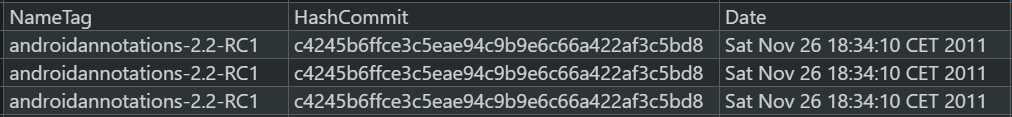
\includegraphics[width=8cm]{img/colonneAggiunte.PNG}
    \caption{Example of the three added column}
    \label{fig:rowAdditional}
\end{figure}

Unfortunately, during the mining, there were some problems with the computation of Designite for some projects, because it could not detect smells and for this reason, they were put aside. There were some problems with VITRuM too and in particular, we couldn't analyze some projects because they didn't have test cases and so there was nothing to analyze or some projects didn't have the correct structure \verb|src/test| that VITRuM finds with the aim of analyzing the projects. The problem of the structure was present when the project was organized in modules, and to resolve this we created a recursive function that analyzed these modules and runs VITRuM on single modules, after that the results were merged all in one. In some other cases, some projects did not have the test folder called \verb|test|, for example, they had \verb|testRun| or similar, and so VITRuM couldn't find it and consequently couldn't analyze the test cases of these projects.
For these reasons, the number of projects passed from 90 to 40, but fortunately, it was not a small number, especially because we selected only big projects with a minimum of 10 releases, and it allowed us to conduct the analysis of the resultant data.

% !TeX spellcheck = en_US
\section{Analysis of Results}\label{sec:results}

After collecting all the data of the Architectural and Test smells we analyzed them. This section discusses the obtained results with the goal of answering the two formulated questions. In particular, we will present the findings for Q1 in Section 3.1 and Q2 in Section 3.2 to facilitate discussion of the results and avoid redundancies.

\subsection{Q1: Correlated increase of Architectural and Test smells}
For every project that we mined and gathered data we compared this data and created a pair of plots, in particular:
\begin{itemize}
  \item The first represents the number of Architectural Smells for the entire project.
  \item The second represents the number of Test Smells for the entire project.
\end{itemize}
The goal of this phase was to observe visually that with an increase of the number of Architectural Smells for the project there was an increase of Test Smells too.

In the images below you can see this parallel increment between the two plots of the same project.

\begin{figure}[htp]
    \centering
    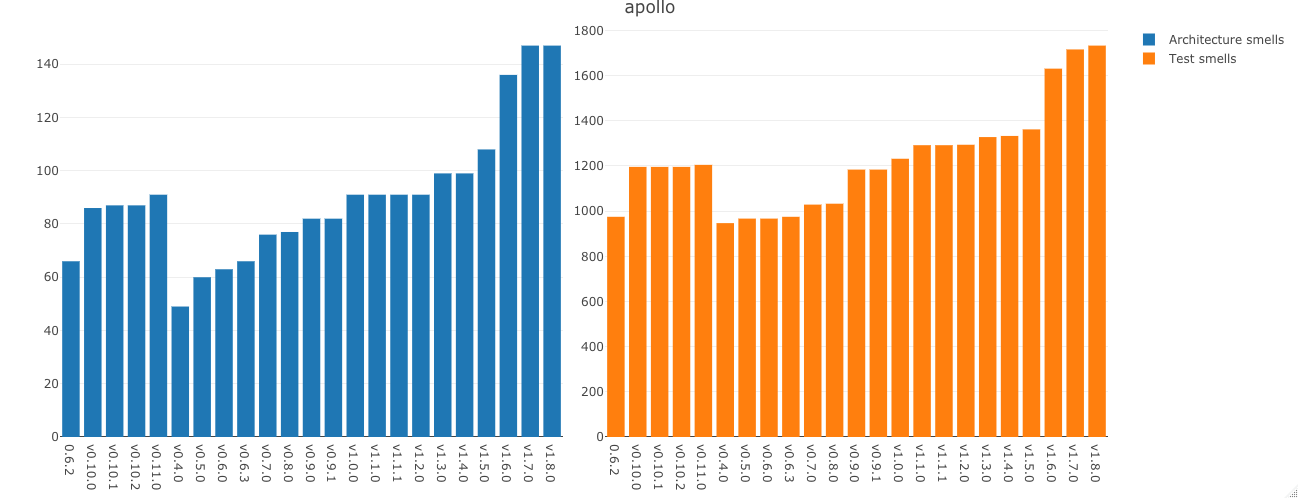
\includegraphics[width=8cm]{img/apollo.png}
    \caption{Project: Apollo}
    \label{fig:apollo}
\end{figure}
\begin{figure}[htp]
    \centering
    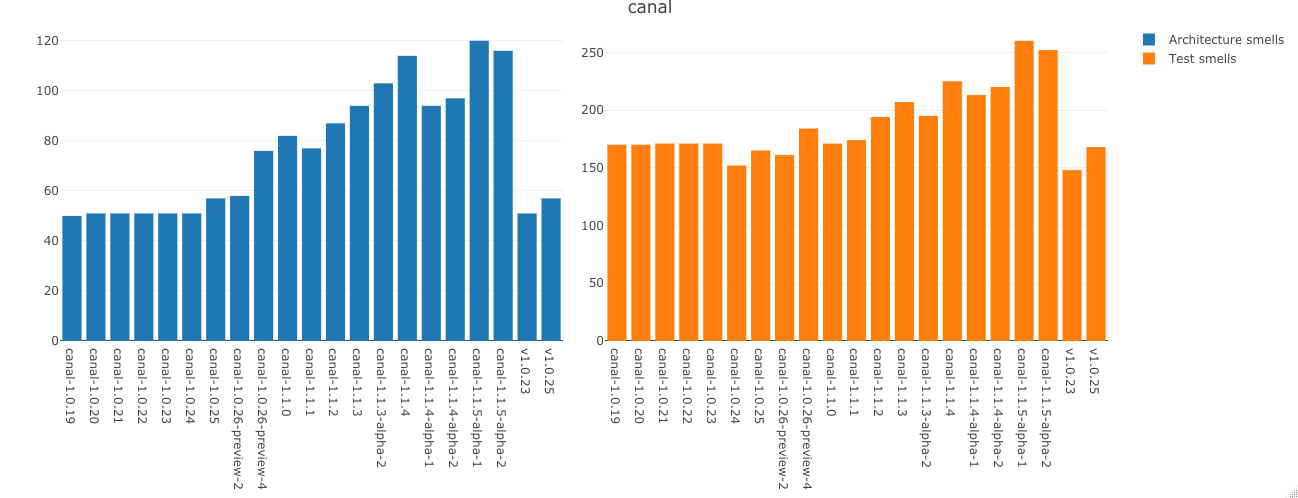
\includegraphics[width=8cm]{img/canal.png}
    \caption{Project: Canal}
    \label{fig:canal}
\end{figure}
\begin{figure}[htp]
    \centering
    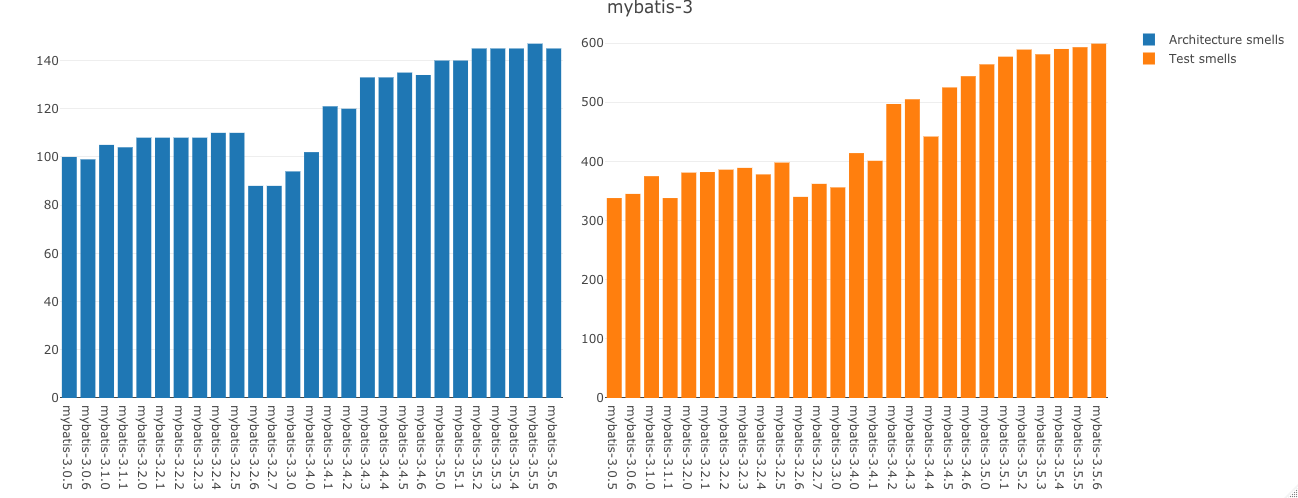
\includegraphics[width=8cm]{img/mybatis-3.png}
    \caption{Project: Mybatis-3}
    \label{fig:mybatis-3}
\end{figure}

For reason of space we reported only a few of the plots of the projects analyzed, but all the other plots are available on the Github repository \cite{IEEEhowto:plotsR}. \par\hfill

As you can observe from the previous plots when there is an increase of Architectural smells (blue plots) there is an increase of Test smells (orange plots) too, and it is also interesting to observe that when the Architectural smells decrease there is a decrease of the Test smells too.\par\hfill

These plots are related to the versions of the projects, so every bar of these represent the number of smells contained in the relative version, while the Architectural smells considered are package-level.\par\hfill

Once computed these, we decided to compute the co-occurrence of the smells\footnote{The counting of paired data within a collection.}, in particular we calculated all the co-occurrence between:
\begin{itemize}
  \item \textit{Architectural Smells - Architectural Smells};
  \item \textit{Test Smells - Test Smells};
  \item \textit{Architectural Smells - Test Smells};
\end{itemize}
As you can see in the Table \ref{co-occurrencesAS} the Architectural Smells considered are at the class level because we compared them with Test Smells that are at a class level too.
In the Table \ref{co-occurrencesTS} there are the co-occurrence of Test Smells, and in the table \ref{co-occurrencesAS-TS} there are the co-occurrence between the Architectural Smells and Test Smells at class level.
The tables in the examples refers to the specific project \textit{"Apollo"} \cite{IEEEhowto:apollo}. 
In the GitHub repository are available the Python scripts to compute it and the result of the computation for all the projects \cite{IEEEhowto:co-occurrence}.

\begin{table}[!ht]
\centering
\caption{Co-occurrences Architectural Smell - Architectural Smell in \emph{Apollo} project.}\label{co-occurrencesAS}
\resizebox{0.5\textwidth}{!}{%
\begin{tabular}{cccccc}
 \csvreader[
  tabular=|r|*{12}{c}|,
  nohead,column count=13,
  table head=\hline,
  late after first line=\\\hline,
  table foot=\hline]{table/apolloArch.csv}%
{}%
{\csviffirstrow{%
  \csvcoli & \myrot{ii} & \myrot{iii} & \myrot{iv} & \myrot{v} & \myrot{vi} & \myrot{vii}
  & \myrot{viii} & \myrot{ix} & \myrot{x} & \myrot{xi} & \myrot{xii} & \myrot{xiii}
}{\csvlinetotablerow}}
\end{tabular}
}
\end{table}

\begin{table}[!ht]
\caption{Co-occurrences Test Smell - Test Smell in \emph{Apollo} project.}\label{co-occurrencesTS}
\resizebox{0.5\textwidth}{!}{%
\begin{tabular}{cccccc}
\csvreader[
  tabular=|r|*{7}{c}|,
  nohead,column count=8,
  table head=\hline,
  late after first line=\\\hline,
  table foot=\hline]{table/apolloTest.csv}%
{}%
{\csviffirstrow{%
  \csvcoli & \myrot{ii} & \myrot{iii} & \myrot{iv} & \myrot{v} & \myrot{vi} & \myrot{vii}
  & \myrot{viii}
}{\csvlinetotablerow}}
\end{tabular}
}
\end{table}

\begin{table}[!ht]
\caption{Co-occurrences Architectural Smell - Test Smell in \emph{Apollo} project.}\label{co-occurrencesAS-TS}
\resizebox{0.5\textwidth}{!}{%
\begin{tabular}{cccccc}
\csvreader[
  tabular=|r|*{7}{c}|,
  nohead,column count=8,
  table head=\hline,
  late after first line=\\\hline,
  table foot=\hline]{table/apolloArchTest.csv}%
{}%
{\csviffirstrow{%
  \csvcoli & \myrot{ii} & \myrot{iii} & \myrot{iv} & \myrot{v} & \myrot{vi} & \myrot{vii}
  & \myrot{viii}
}{\csvlinetotablerow}}
\end{tabular}
}
\end{table}\mbox{}



The Table \ref{co-occurrencesAS} shows clearly that there is the 96\% of probability to find both \emph{Unnecessary Abstraction} and \emph{Unutilized Abstraction}, for example. According to test smells, the table \ref{co-occurrencesTS} shows that there is the 93\% of probability to find \emph{ar1} and \emph{et1} together. Finally, in the table \ref{co-occurrencesAS-TS}, you can see that when there is the smell \emph{Wide Hierarchy} with the 79\% of probability there will be a test smell \emph{ar1}.
\par\hfill

\subsection{Q2: Find association between smells through Association rule}
After that, our goal was to find an association between different objects in a set, find frequent patterns in any information repository. In particular, our purpose was to generate a set of rules called Association Rules, in form \textbf{if this then that}.

Also in this case we considered the three combination of (i) \textit{Architectural Smells - Architectural Smells}, (ii) \textit{Test Smells - Test Smells}, (iii) \textit{Architectural Smells - Test Smells}, where for Architectural Smells we refer to class level.
What we have done here was to create a unique dataset witch contains all the Architectural Smells for all the projects and a unique dataset that contains all the Test Smells for all the projects. After that, we did the inner join between them on the attribute className (in fact for this reason we considered Architectural Smells at class level). The result of this operation was a big dataset that contains for each class several rows with all the smells for all the versions of all the projects. For simplicity in reading, we had added an additional column that contained the smells of that row separated by commas.

Before applying Association Rule mining, we needed to convert data frame into transaction data so that all smells that appeared together in one class were put in one row.
The smells were grouped using NameClass. We did this in R with:

\begin{lstlisting}[language=R]
library(plyr)

transactionData <- ddply(df_join,c("ClassName"),
          function(df_join)paste(df_join$Smells,
                                collapse = ","))
\end{lstlisting}

These data then were saved in a CSV file and then was loaded into an object of the transaction class. This was done by using the R function \verb|read.transactions| with the basket format and converted it into an object of the transaction class. 
With the summary of the transactions we obtained:


\begin{figure}[htp]
    \centering
    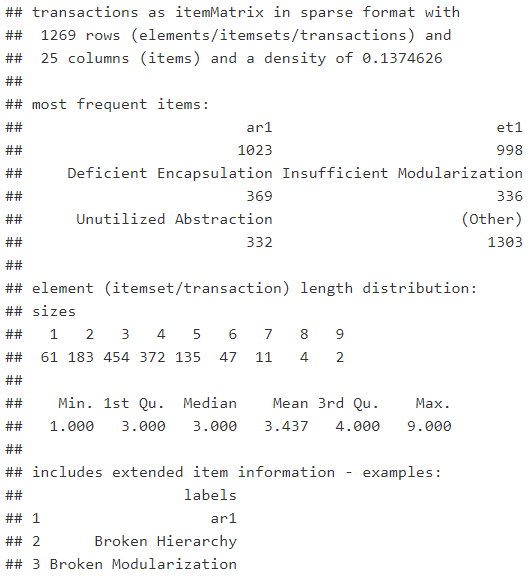
\includegraphics[width=8.5cm]{img/summaryTransaction.PNG}
    \caption{Summary of transaction results}
    \label{fig:summaryTransaction}
\end{figure}

In particular:
\begin{itemize}
  \item There are 1269 transactions (rows) and 25 items (columns). Note that 25 are the smells involved in the dataset and 1269 transactions are collections of these items.
  \item Density tells the percentage of non-zero cells in a sparse matrix. You can say it as the total number of smells that are detected divided by a possible number of smells in that matrix. You can calculate how many items were purchased by using density: $1269 * 25 * 0.1374626 = 4361.0$.
\end{itemize}

Then we computed the item frequency plots for both absolute and relative because if absolute it will plot numeric frequencies of each item independently, if relative it will plot how many times these items have appeared as compared to others. 
\begin{figure}[htp]
    \centering
    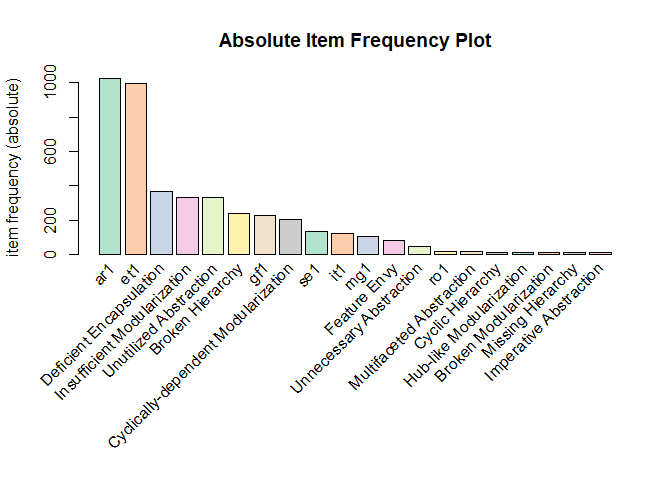
\includegraphics[width=8.5cm]{img/absoluteItemFreq.png}
    \caption{Absolute Item Frequency Plot}
    \label{fig:absoluteItemFreq}
\end{figure}
\begin{figure}[htp]
    \centering
    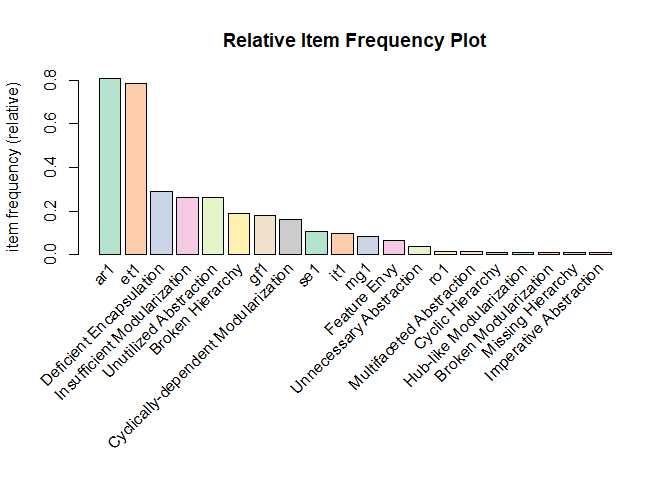
\includegraphics[width=8.5cm]{img/relativeItemFreq.png}
    \caption{Relative Item Frequency Plot}
    \label{fig:relativeItemFreq}
\end{figure}

The next step was to mine the rules using the \textbf{APRIORI} algorithm. We used the function \verb|apriori()| from package \verb|arules|. The apriori takes the transaction data as the transaction object on which mining is to be applied. The parameter that we used for the support was 0.001, and for the confidence was 0.8 (because several works have chosen these thresholds  like \cite{IEEEhowto:associationRules}), then we specified a maximum of 2 items (maxlen), minimum of 2 items (minlen). With the appearance, we specified the LHS (IF part) with the array of Architectural Smells and RHS (THEN part) with the Test Smells.

\begin{lstlisting}[language=R]
design_smells = c('Deficient Encapsulation', 'Unutilized Abstraction', 'Feature Envy',  'Broken Hierarchy', 'Broken Modularization', 'Insufficient Modularization', 'Wide Hierarchy', 'Unnecessary Abstraction', 'Multifaceted Abstraction', 'Cyclically-dependent Modularization','Cyclic Hierarchy', 'Rebellious Hierarchy')

test_smells = c("ar1", "et1", "it1",  "gf1", "se1", "mg1", "ro1")

association.rules <- 
apriori(tr, parameter = list(supp=0.001,                          conf=0.8, minlen=2, maxlen=2),
    appearance = list(lhs=design_smells, rhs=test_smells))
\end{lstlisting}

From this computation with these parameters we obtained 9 rules.


\begin{figure}[htp]
    \centering
    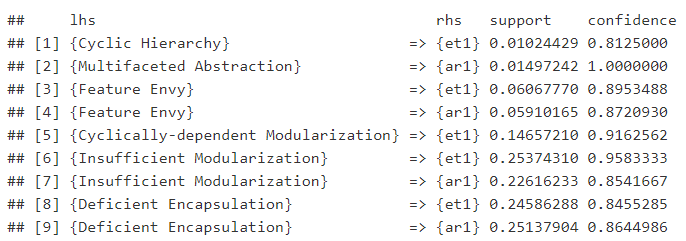
\includegraphics[width=8.5cm]{img/ruleArchTest.PNG}
    \caption{Rule Architectural Smells - Test Smells}
    \label{fig:ruleArchTest}
\end{figure}

Using the above output, you can make analyses such as:
\begin{itemize}
  \item Classes which have design smell \textit{‘Cyclic Hierarchy’} will have the test smell \textit{‘et1’} with support of 0.01 and confidence of 0.81.
  \item Classes which have design smell \textit{‘Multifaceted Abstraction’} will have the test smell \textit{‘ar1’} with support of 0.0149 and confidence of 1.
  \item Classes which have design smell \textit{‘Feature Envy’} will have the test smell \textit{‘et1’} with support of 0.06 and confidence of 0.89.
  \item Classes which have design smell \textit{‘Feature Envy’} will have the test smell \textit{‘ar1’} with support of 0.059 and confidence of 0.87.
\end{itemize}

We did the same thing with both LHS (left part) and RHS (right part) imposed with Architectural Smells, but here we setted the parameter maxlen of the apriori function equals to 4 because with maxlen=2 or maxlen=3 there were less then 2 rules. From this computation we obtained the following 7 rules: \par
\begin{figure}[htp]
    \centering
    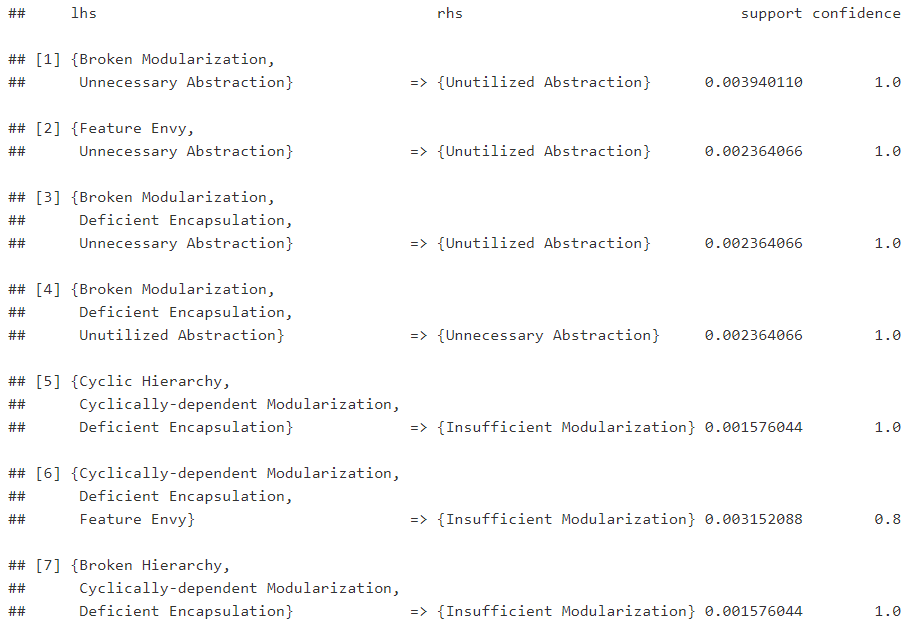
\includegraphics[width=8.5cm]{img/ruleArch.PNG}
    \caption{Rule Architectural Smells - Architectural Smells}
    \label{fig:ruleArch}
\end{figure}
Using the above output, you can make analyses such as:
\begin{itemize}
  \item Classes which have design smells \textit{‘Broken Modularization’} and \textit{‘Unnecessary Abstraction’} will have the design smell \textit{‘Unutilized Abstraction’} with support of 0.0039 and confidence of 1.
  \item Classes which have design smell \textit{‘Feature Envy’} and ‘Unnecessary Abstraction’ will have the design smell \textit{‘Unutilized Abstraction’} with support of 0.0023 and confidence of 1.
\end{itemize}

Finally, we did the same computation to Test Smells to and we called the apriori function with both LHS (left part) and RHS (right part) imposed with Test Smells but here we imposed the maxlen and minlen both equals to 2. From this computation, we obtained 13 rules and we filtered the first 10:
\begin{figure}[htp]
    \centering
    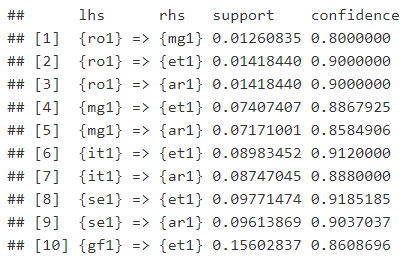
\includegraphics[width=8.5cm]{img/ruleTest.PNG}
    \caption{Rule Test Smells - Test Smells}
    \label{fig:ruleTest}
\end{figure}

Using the above output, you can make analyses such as:
\begin{itemize}
  \item Classes which have test smell \textit{‘ro1’} will have the test smell \textit{‘mg1’} with support of 0.0126 and confidence of 0.8.
  \item Classes which have test smell \textit{‘ro1’} will have the test smell \textit{‘et1’} with support of 0.0141 and confidence of 0.9.
\end{itemize}
\par\hfill

\subsubsection{Visualize Association Rules}

Since there will be hundreds or thousands of rules generated based on data, there are a couple of ways to visualize these association rules.
%\begin{figure}[ht]
%    \centering
%    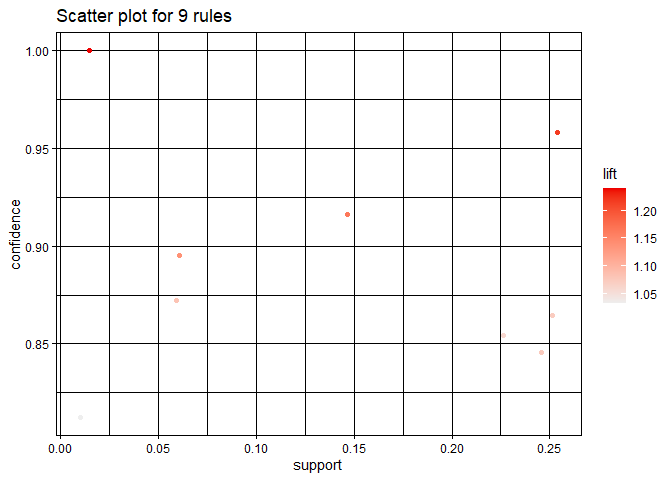
\includegraphics[width=5cm]{img/scatterPlotArchTest.png}
%    \caption{Scatter-Plot Architectural Smells-Test Smell}
%    \label{fig:scatterPlotArchTest}
%\end{figure}
%\begin{figure}[ht]
%    \centering
%    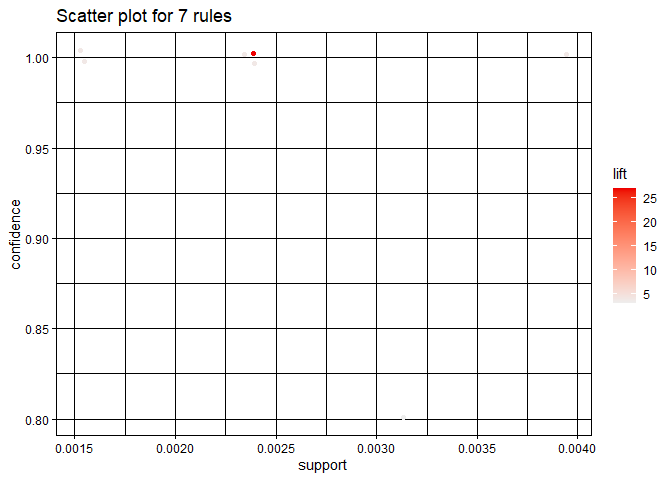
\includegraphics[width=5cm]{img/scatterPlotArch.png}
%    \caption{Scatter-Plot Architectural Smells}
%    \label{fig:scatterPlotArch}
%\end{figure}
%\begin{figure}[ht]
%    \centering
%    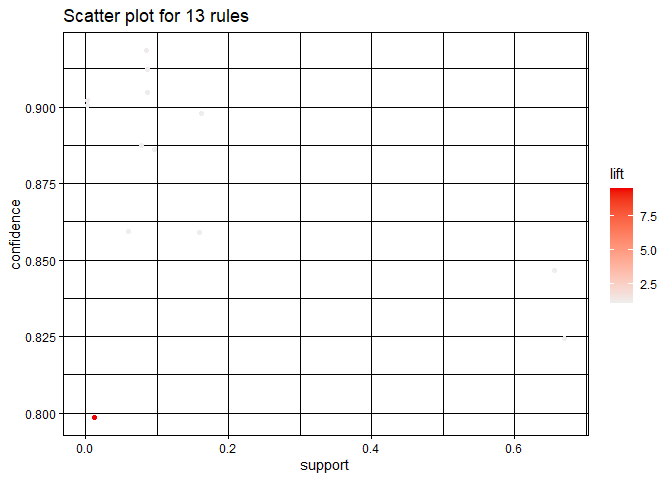
\includegraphics[width=5cm]{img/scatterPlotTest.png}
%    \caption{Scatter-Plot Test Smells}
%    \label{fig:scatterPlotTest}
%\end{figure}

One of the visualization that we computed is the Individual Rule Representation, this representation is also called as Parallel Coordinates Plot.
\begin{figure}[!ht]
    \centering
    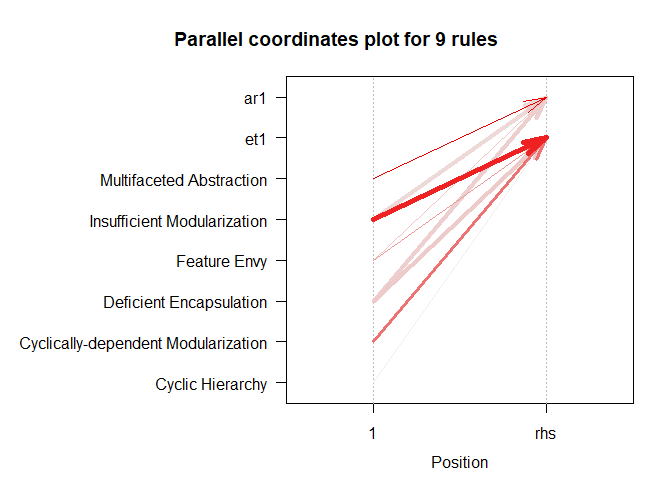
\includegraphics[width=5cm]{img/parallelCoordinateArchTest.png}
    \caption{Parallel Coordinate Architectural Smells-Test Smell}
    \label{fig:parallelCoordinateArchTest}
\end{figure}
\begin{figure}[!ht]
    \centering
    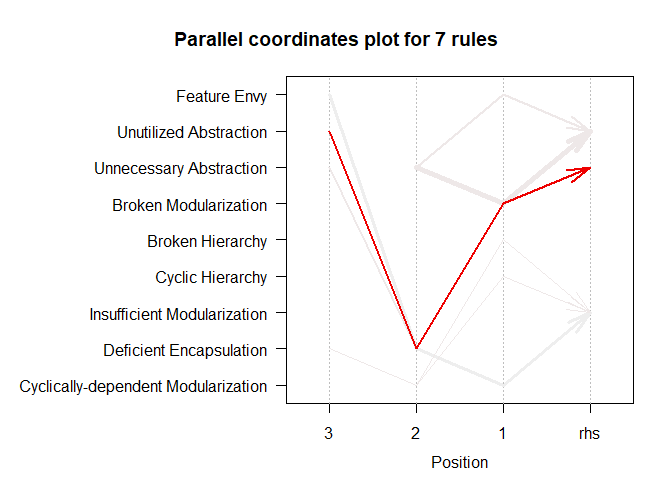
\includegraphics[width=5cm]{img/parallelCoordinateArch.png}
    \caption{Parallel Coordinate Architectural Smells}
    \label{fig:parallelCoordinateArch}
\end{figure}
\begin{figure}[!ht]
    \centering
    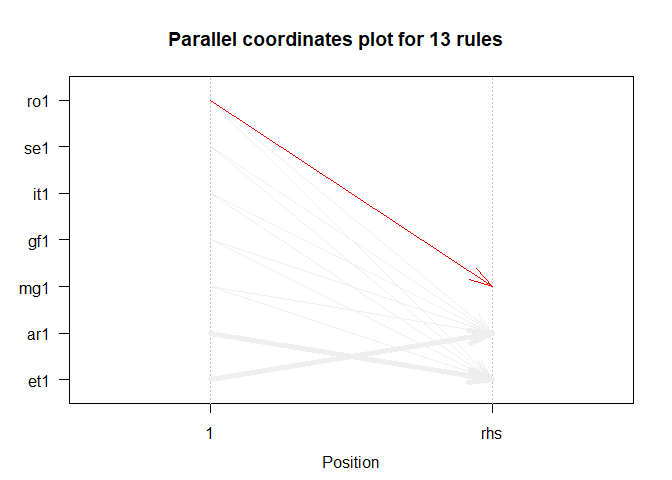
\includegraphics[width=5cm]{img/parallelCoordinateTest.png}
    \caption{Parallel Coordinate Test Smells}
    \label{fig:parallelCoordinateTest}
\end{figure}

For example, Figure \ref{fig:parallelCoordinateTest} shows that when the class has the test smell \textit{'ro1'}, with high probability it will also have the test smell \textit{'mg1'}.
All these plots have been created throw R, the scripts and a report of these results are all reported on GitHub \cite{IEEEhowto:rNotebook}.\par\hfill\par\hfill\par\hfill\par\hfill

% !TeX spellcheck = en_US
\section{Discussion}\label{sec:discussion}
% !TeX spellcheck = en_US
\section{Conclusion}\label{sec:conclusion}

\IEEEPARstart{B}{oth} Architectural and Test smells, as smells are symptoms of poor design or implementation choices. What we wanted to present in this project was a relationship between the Architectural smells and Test smells, in particular, in the first moment we computed the co-occurrences among them for all the smells of the projects that we selected and mined on GitHub, by providing evidence on what are the smells that co-occur more frequently not only among Architectural-Test but also between Architectural-Architectural and Test-Test smells.

After that our focus was on the Association Rule because our principal purpose was to show that the introduction of an Architectural smell increase the difficulty to write the relative test case, because of the complexity of the structure of the code to test, and therefore the developer while testing these smelly components will introduce some Test smells. At this point, we computed the Association Rule, through the Apriori function, on all the smells of the projects that we collected, to discover what Architectural smell lead to what Test smell and what is its support and its confidence. What we concluded was that various Architectural smell lead more frequency to the Test smell \textit{"ar"} and \textit{"et"}. We computed also the Association rule between the Architectural-Architectural and Test-Test smells.

These findings represent the main results of our project, but also some other researches could be done to discover eventually other rules of Association Rule by considering new Architectural smells and Test smells in addition to those already considered.



% use section* for acknowledgment
\ifCLASSOPTIONcompsoc
  % The Computer Society usually uses the plural form
  \section*{Acknowledgments}
\else
  % regular IEEE prefers the singular form
  \section*{Acknowledgment}
\fi


The authors would like to thank...


% Can use something like this to put references on a page
% by themselves when using endfloat and the captionsoff option.
\ifCLASSOPTIONcaptionsoff
  \newpage
\fi



% trigger a \newpage just before the given reference
% number - used to balance the columns on the last page
% adjust value as needed - may need to be readjusted if
% the document is modified later
%\IEEEtriggeratref{8}
% The "triggered" command can be changed if desired:
%\IEEEtriggercmd{\enlargethispage{-5in}}

% references section

% can use a bibliography generated by BibTeX as a .bbl file
% BibTeX documentation can be easily obtained at:
% http://mirror.ctan.org/biblio/bibtex/contrib/doc/
% The IEEEtran BibTeX style support page is at:
% http://www.michaelshell.org/tex/ieeetran/bibtex/
%\bibliographystyle{IEEEtran}
% argument is your BibTeX string definitions and bibliography database(s)
%\bibliography{IEEEabrv,../bib/paper}
%
% <OR> manually copy in the resultant .bbl file
% set second argument of \begin to the number of references
% (used to reserve space for the reference number labels box)
\begin{thebibliography}{1}

\bibitem{IEEEhowto:kopka}
H.~Kopka and P.~W. Daly, \emph{A Guide to \LaTeX}, 3rd~ed.\hskip 1em plus
  0.5em minus 0.4em\relax Harlow, England: Addison-Wesley, 1999.

\end{thebibliography}

% biography section
% 
% If you have an EPS/PDF photo (graphicx package needed) extra braces are
% needed around the contents of the optional argument to biography to prevent
% the LaTeX parser from getting confused when it sees the complicated
% \includegraphics command within an optional argument. (You could create
% your own custom macro containing the \includegraphics command to make things
% simpler here.)
%\begin{IEEEbiography}[{\includegraphics[width=1in,height=1.25in,clip,keepaspectratio]{mshell}}]{Michael Shell}
% or if you just want to reserve a space for a photo:

%\begin{IEEEbiography}{Michael Shell}
%Biography text here.
%\end{IEEEbiography}
%
%% if you will not have a photo at all:
%\begin{IEEEbiographynophoto}{John Doe}
%Biography text here.
%\end{IEEEbiographynophoto}
%
%% insert where needed to balance the two columns on the last page with
%% biographies
%%\newpage
%
%\begin{IEEEbiographynophoto}{Jane Doe}
%Biography text here.
%\end{IEEEbiographynophoto}

% You can push biographies down or up by placing
% a \vfill before or after them. The appropriate
% use of \vfill depends on what kind of text is
% on the last page and whether or not the columns
% are being equalized.

%\vfill

% Can be used to pull up biographies so that the bottom of the last one
% is flush with the other column.
%\enlargethispage{-5in}



% that's all folks
\end{document}


